% questions.tex —— 2016 年·北京卷·文科 · 题目内容片段（无答案）
% 由 tools/generate_projects.py 依来源总账自 2016/2016_数学真题_北京文_试题.md 生成，勿手改（改源 MD 后重跑）


\gkpart{数学}

\begin{gktip}
\textbf{来源说明}：本题面依据固定源 PDF 两页 A3 页面逐题核对，原卷印刷页码 995–996。固定源不附答案；本文件仅为题面规范源。
\end{gktip}

\gkpart{一、选择题}

\begin{question}
\gkti{1}已知集合 \(A=\{x\mid 2<x<4\}\)，\(B=\{x\mid x<3\) 或 \(x>5\}\)，则 \(A\cap B=\)（　）

（A）\(\{x\mid 2<x<5\}\)　（B）\(\{x\mid x<4\) 或 \(x>5\}\)

（C）\(\{x\mid 2<x<3\}\)　（D）\(\{x\mid x<2\) 或 \(x>5\}\)

\end{question}
\begin{question}
\gkti{2}复数 \(\dfrac{1+2\mathrm{i}}{2-\mathrm{i}}=\)（　）

（A）\(\mathrm{i}\)　（B）\(1+\mathrm{i}\)　（C）\(-\mathrm{i}\)　（D）\(1-\mathrm{i}\)

\Needspace{0.4\textheight}
\end{question}
\begin{question}
\gkti{3}执行如图所示的程序框图，输出的 \(s\) 值为（　）
\nopagebreak[4]
\begin{center}% 第 3 题程序框图：按固定源 PDF 的框图结构逐一重绘（框形、分支标签与回边走向照原图）。
% 回边次序（易错点，600 dpi 逐箭头核对）：「是」分支先进入 \(s=s+k^{3}\)（箭头指向其下沿），
% 再上行进入 \(k=k+1\)，最后由 \(k=k+1\) 顶边折回主干，箭头指向主干（T 形汇入）。
% 坐标全部显式给定：主干 x=0；回边列 x=-3.4；join 在 init 底边下 0.35cm；
% inc 顶边(-2.6) 与 init 底边(-1.4) 留 1.2cm 空档，杜绝框体重叠与回边穿框。
\begin{tikzpicture}[>=stealth,every node/.style={font=\small},
  term/.style={draw,rounded corners,minimum width=1.5cm,minimum height=6mm},
  box/.style={draw,minimum width=2.2cm,minimum height=6mm},
  io/.style={draw,trapezium,trapezium left angle=70,trapezium right angle=110,minimum width=1.9cm,minimum height=6mm},
  decision/.style={draw,diamond,aspect=2.6,minimum width=2.6cm,minimum height=1.0cm,inner sep=0pt}]
\node[term] (start) at (0,0) {开始};
\node[box] (init) at (0,-1.1) {\(k=0,\ s=0\)};
\node[decision] (test) at (0,-6.6) {\(k\leqslant 2\)};
\node[io] (out) at (0,-8.0) {输出 \(s\)};
\node[term] (end) at (0,-9.2) {结束};
\node[box] (inc) at (-3.4,-2.9) {\(k=k+1\)};
\node[box] (add) at (-3.4,-4.5) {\(s=s+k^{3}\)};
\coordinate (join) at (0,-1.75);
\draw[->] (start)--(init);
\draw[->] (init)--(test);
\draw[->] (test.south)--node[right,xshift=2pt]{否}(out.north);
\draw[->] (out)--(end);
\draw[->] (test.west) -| node[above,pos=0.35]{是} (add.south);
\draw[->] (add.north)--(inc.south);
\draw[->] (inc.north) |- (join);
\end{tikzpicture}
\end{center}
\nopagebreak[4]
（A）\(8\)　（B）\(9\)　（C）\(27\)　（D）\(36\)

\end{question}
\begin{question}
\gkti{4}下列函数中，在区间 \((-1,1)\) 上为减函数的是（　）

（A）\(y=\dfrac{1}{1-x}\)　（B）\(y=\cos x\)　（C）\(y=\ln(x+1)\)　（D）\(y=2^{-x}\)

\end{question}
\begin{question}
\gkti{5}圆 \((x+1)^{2}+y^{2}=2\) 的圆心到直线 \(y=x+3\) 的距离为（　）

（A）\(1\)　（B）\(2\)　（C）\(\sqrt{2}\)　（D）\(2\sqrt{2}\)

\end{question}
\begin{question}
\gkti{6}从甲、乙等 \(5\) 名学生中随机选出 \(2\) 人，则甲被选中的概率为（　）

（A）\(\dfrac{1}{5}\)　（B）\(\dfrac{2}{5}\)　（C）\(\dfrac{8}{25}\)　（D）\(\dfrac{9}{25}\)

\end{question}
\begin{question}
\gkti{7}已知 \(A(2,5)\)，\(B(4,1)\)。若点 \(P(x,y)\) 在线段 \(AB\) 上，则 \(2x-y\) 的最大值为（　）

（A）\(-1\)　（B）\(3\)　（C）\(7\)　（D）\(8\)

\end{question}
\begin{question}
\gkti{8}某学校运动会的立定跳远和 \(30\) 秒跳绳两个单项比赛分成预赛和决赛两个阶段，下表为 \(10\) 名学生的预赛成绩，其中有三个数据模糊。

\begin{center}
\begin{tabular}{llllll}
\toprule
学生序号 & \(1\) & \(2\) & \(3\) & \(4\) & \(5\) \\
\midrule
立定跳远（单位：米） & \(1.96\) & \(1.92\) & \(1.82\) & \(1.80\) & \(1.78\) \\
\(30\) 秒跳绳（单位：次） & \(63\) & \(a\) & \(75\) & \(60\) & \(63\) \\
学生序号 & \(6\) & \(7\) & \(8\) & \(9\) & \(10\) \\
立定跳远（单位：米） & \(1.76\) & \(1.74\) & \(1.72\) & \(1.68\) & \(1.60\) \\
\(30\) 秒跳绳（单位：次） & \(72\) & \(70\) & \(a-1\) & \(b\) & \(65\) \\
\bottomrule
\end{tabular}
\end{center}

在这 \(10\) 名学生中，进入立定跳远决赛的有 \(8\) 人，同时进入立定跳远决赛和 \(30\) 秒跳绳决赛的有 \(6\) 人，则（　）

（A）\(2\) 号学生进入 \(30\) 秒跳绳决赛　（B）\(5\) 号学生进入 \(30\) 秒跳绳决赛

（C）\(8\) 号学生进入 \(30\) 秒跳绳决赛　（D）\(9\) 号学生进入 \(30\) 秒跳绳决赛

\end{question}
\gkpart{二、填空题}

\begin{question}
\gkti{9}已知向量 \(\boldsymbol{a}=(1,\sqrt{3})\)，\(\boldsymbol{b}=(\sqrt{3},1)\) 则 \(\boldsymbol{a}\) 与 \(\boldsymbol{b}\) 夹角的大小为 \(\underline{\qquad}\)。

\end{question}
\begin{question}
\gkti{10}函数 \(f(x)=\dfrac{x}{x-1}\)（\(x\geqslant 2\)）的最大值为 \(\underline{\qquad}\)。

\Needspace{0.4\textheight}
\end{question}
\begin{question}
\gkti{11}某四棱柱的三视图如图所示，则该四棱柱的体积为 \(\underline{\qquad}\)。
\nopagebreak[4]
\begin{center}% 第 11 题四棱柱三视图：按固定源 PDF 的视图排布与尺寸线位置重绘（数字只保留原图印出的 1、1、1、2）。
% 正（主）视图为 2:1 矩形、内部两条竖直虚线在宽度的 1/4 与 3/4 处（梯形两斜棱的投影），原图无尺寸标注。
% 俯视图整块较视图标签下移 0.5cm：标签（锚 y=-0.32，字高约 0.37）与上底尺寸线（y=-1.12）留出 0.43cm 白隙。
\begin{tikzpicture}[every node/.style={font=\small},scale=0.9,line cap=round,line join=round]
% 正（主）视图：矩形内两条竖直虚线，无尺寸标注
\draw (0,0) rectangle (2.0,1.0);
\draw[dashed] (0.5,0)--(0.5,1.0);
\draw[dashed] (1.5,0)--(1.5,1.0);
\node[below] at (1.0,-0.32) {正（主）视图};
% 侧（左）视图：正方形；右侧竖直尺寸线（两端端线），数字 1 在旁
\draw (3.3,0) rectangle (4.3,1.0);
\draw[<->] (4.68,0)--(4.68,1.0);
\draw (4.55,0)--(4.81,0); \draw (4.55,1.0)--(4.81,1.0);
\node[right] at (4.85,0.5) {\(1\)};
\node[below] at (3.8,-0.32) {侧（左）视图};
% 俯视图：等腰梯形（上底 1、下底 2、高 1）；上底上方数字 1 断开的水平尺寸线，
% 右侧竖直尺寸线旁标 1，下底下方数字 2 断开的水平尺寸线
\draw (0,-2.4)--(2.0,-2.4)--(1.5,-1.4)--(0.5,-1.4)--cycle;
\draw[<->] (0.5,-1.12)--(1.5,-1.12);
\node[fill=white,inner sep=1.2pt] at (1.0,-1.12) {\(1\)};
\draw[<->] (2.42,-1.4)--(2.42,-2.4);
\draw (2.29,-1.4)--(2.55,-1.4); \draw (2.29,-2.4)--(2.55,-2.4);
\node[right] at (2.58,-1.9) {\(1\)};
\draw[<->] (0,-2.68)--(2.0,-2.68);
\node[fill=white,inner sep=1.2pt] at (1.0,-2.68) {\(2\)};
\node[below] at (1.0,-3.05) {俯视图};
\end{tikzpicture}
\end{center}
\nopagebreak[4]
\end{question}
\begin{question}
\gkti{12}已知双曲线 \(\dfrac{x^{2}}{a^{2}}-\dfrac{y^{2}}{b^{2}}=1\)（\(a>0\)，\(b>0\)）的一条渐近线为 \(2x+y=0\)，一个焦点为 \((\sqrt{5},0)\)，则 \(a=\underline{\qquad}\)；\(b=\underline{\qquad}\)。

\end{question}
\begin{question}
\gkti{13}在 \(\triangle ABC\) 中，\(\angle A=\dfrac{2\pi}{3}\)，\(a=\sqrt{3}c\)，则 \(\dfrac{b}{c}=\underline{\qquad}\)。

\end{question}
\begin{question}
\gkti{14}某网店统计了连续三天售出商品的种类情况：第一天售出 \(19\) 种商品，第二天售出 \(13\) 种商品，第三天售出 \(18\) 种商品；前两天都售出的商品有 \(3\) 种，后两天都售出的商品有 \(4\) 种，则该网店

① 第一天售出但第二天未售出的商品有 \(\underline{\qquad}\) 种；

② 这三天售出的商品最少有 \(\underline{\qquad}\) 种。

\end{question}
\gkpart{三、解答题}

\begin{question}
\gkti{15}已知 \(\{a_{n}\}\) 是等差数列，\(\{b_{n}\}\) 是等比数列，且 \(b_{2}=3\)，\(b_{3}=9\)，\(a_{1}=b_{1}\)，\(a_{14}=b_{4}\)。

（1） 求 \(\{a_{n}\}\) 的通项公式；

（2） 设 \(c_{n}=a_{n}+b_{n}\)，求数列 \(\{c_{n}\}\) 的前 \(n\) 项和。

\end{question}
\begin{question}
\gkti{16}已知函数 \(f(x)=2\sin\omega x\cos\omega x+\cos 2\omega x\)（\(\omega>0\)）的最小正周期为 \(\pi\)。

（1） 求 \(\omega\) 的值；

（2） 求 \(f(x)\) 的单调递增区间。

\Needspace{0.4\textheight}
\end{question}
\begin{question}
\gkti{17}某市居民用水拟实行阶梯水价，每人每月用水量中不超过 \(w\) 立方米的部分按 \(4\) 元/立方米收费，超出 \(w\) 立方米的部分按 \(10\) 元/立方米收费，从该市随机调查了 \(10000\) 位居民，获得了他们某月的用水量数据，整理得到如图频率分布直方图：
\nopagebreak[4]
\begin{center}% 第 17 题频率分布直方图：柱高按固定源 PDF 像素实测重绘（组距 0.5，共 9 组）。
% 最左组 [0,0.5) 频率为 0（原图如此）：纵轴与第一根柱之间留一个组距空档，不画柱。
\begin{tikzpicture}[>=stealth,every node/.style={font=\small}]
\def\ux{1.15}   % 横轴：1 立方米
\def\uy{3.6}    % 纵轴：单位 1（频率/组距）
% 坐标轴（横轴标题置于轴箭头右端之后，与原图一致；不可用 below left 锚到 (5.45,0)——会覆盖 2.5–4.5 刻度）
\draw[->] (0,0)--(5.45,0) node[right,yshift=-2pt] {用水量（立方米）};
\draw[->] (0,0)--(0,2.05);
\node[anchor=south west] at (0.10,2.02) {\begin{tabular}{c}频率\\\hline 组距\end{tabular}};
% 刻度虚线（0.1–0.5）与纵轴刻度标签
\foreach \v in {0.1,0.2,0.3,0.4,0.5} {
  \draw[dashed] (0,\v*\uy)--(5.1,\v*\uy);
  \node[left] at (-0.08,\v*\uy) {\(\v\)};
}
% 横轴刻度标签
\foreach \t in {0,0.5,1,1.5,2,2.5,3,3.5,4,4.5} {
  \node[below] at (\t*\ux,-0.10) {\(\t\)};
}
% 柱（空心矩形，相邻柱共用竖边；最左组无柱）：
% [0.5,1)=0.2，[1,1.5)=0.3，[1.5,2)=0.4，[2,2.5)=0.5，[2.5,3)=0.3，[3,3.5)=[3.5,4)=[4,4.5)=0.1
\foreach \i/\h in {1/0.2, 2/0.3, 3/0.4, 4/0.5, 5/0.3, 6/0.1, 7/0.1, 8/0.1} {
  \draw ({0.5*\i*\ux},0) rectangle ({0.5*(\i+1)*\ux},{\h*\uy});
}
\end{tikzpicture}
\end{center}
\nopagebreak[4]
（1） 如果 \(w\) 为整数，那么根据此次调查，为使 80\% 以上居民在该月的用水价格为 \(4\) 元/立方米，\(w\) 至少定为多少？

（2） 假设同组中的每个数据用该组区间的右端点值代替，当 \(w=3\) 时，估计该市居民该月的人均水费。

\Needspace{0.4\textheight}
\end{question}
\begin{question}
\gkti{18}如图，在四棱锥 \(P-ABCD\) 中，\(PC\perp\) 平面 \(ABCD\)，\(AB\parallel DC\)，\(DC\perp AC\)。
\nopagebreak[4]
\begin{center}% 第 18 题四棱锥 P-ABCD：按固定源 PDF 的顶点相对位置重绘。
% 实线 5 条：PA、PB、PD、DA、AB；虚线 4 条：PC（棱锥的高）、CD、CB、CA。
% 虚线 CB 与实线 PA 在投影中相交（900 dpi 核对：PB 之外唯一交叉，实线压在上层）——先画虚线后画实线即得。
% E 为 AB 中点（实心圆点），与原题「E 为 AB 的中点」一致。
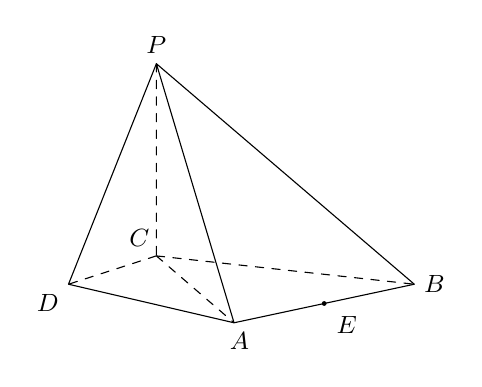
\begin{tikzpicture}[line cap=round,line join=round,font=\small,scale=0.72]
\coordinate (P) at (1.60,4.60);
\coordinate (C) at (1.60,1.21);
\coordinate (D) at (0.05,0.71);
\coordinate (B) at (6.15,0.71);
\coordinate (A) at (2.97,0.03);
\coordinate (E) at (4.56,0.37);
% 虚线先画（含 PC 竖线与底面后侧棱、对角线 CA）
\draw[dashed] (P)--(C) (C)--(D) (C)--(B) (C)--(A);
% 实线后画（压住虚线交叉处，与原图一致）
\draw (P)--(D) (P)--(B) (P)--(A) (D)--(A) (A)--(B);
\node[above] at (P) {$P$};
\node[above left,xshift=1pt] at (C) {$C$};
\node[below left] at (D) {$D$};
\node[right] at (B) {$B$};
\node[below,xshift=2pt] at (A) {$A$};
\fill (E) circle (1.2pt) node[below right,xshift=1pt,yshift=-1pt] {$E$};
\end{tikzpicture}
\end{center}
\nopagebreak[4]
（1） 求证：\(DC\perp\) 平面 \(PAC\)；

（2） 求证：平面 \(PAB\perp\) 平面 \(PAC\)；

（3） 设点 \(E\) 为 \(AB\) 的中点。在棱 \(PB\) 上是否存在点 \(F\)，使得 \(PA\parallel\) 平面 \(CEF\)？说明理由。

\end{question}
\begin{question}
\gkti{19}已知椭圆：\(C:\dfrac{x^{2}}{a^{2}}+\dfrac{y^{2}}{b^{2}}=1\) 过点 \(A(2,0)\)，\(B(0,1)\) 两点。

（1） 求椭圆 \(C\) 的方程及离心率；

（2） 设 \(P\) 为第三象限内一点且在椭圆 \(C\) 上，直线 \(PA\) 与 \(y\) 轴交于点 \(M\)，直线 \(PB\) 与 \(x\) 轴交于点 \(N\)，求证：四边形 \(ABNM\) 的面积为定值。

\end{question}
\begin{question}
\gkti{20}设函数 \(f(x)=x^{3}+ax^{2}+bx+c\)。

（1） 求曲线 \(y=f(x)\) 在点 \((0,f(0))\) 处的切线方程；

（2） 设 \(a=b=4\)，若函数 \(f(x)\) 有三个不同零点，求 \(c\) 的取值范围；

（3） 求证：\(a^{2}-3b>0\) 是 \(f(x)\) 有三个不同零点的必要而不充分条件。

\end{question}